\chapter*{PLANOS Y LÁMINAS DE DETALLE}
\addcontentsline{toc}{chapter}{PLANOS Y LÁMINAS DE DETALLE}

% Reinicio de contadores para numeracion coherente con el capitulo 7.
\setcounter{section}{0}
\renewcommand{\thesection}{7.\arabic{section}.}
\renewcommand{\thesubsection}{7.\arabic{section}.\arabic{subsection}.}
\renewcommand{\theHsection}{planos.\arabic{section}}
\renewcommand{\theHsubsection}{planos.\arabic{section}.\arabic{subsection}}

\section{RELACIÓN DE PLANOS DEL PROYECTO}

Los planos adjuntos forman parte integral de este expediente tecnico y representan la distribucion de salidas de alumbrado, tomacorrientes generales y de fuerza, recorridos de canalizacion, ubicacion de tableros (TG y T2) y el sistema de puesta a tierra.

\begin{table}[H]
\centering
\caption{Relación de planos presentados}
\label{tab:planos-relacion}
\begin{tabularx}{\textwidth}{L c L c}
\toprule
\textbf{Código} & \textbf{Descripción} & \textbf{Archivo de Referencia} & \textbf{Estado} \\
\midrule
IE-01 & Plano de Instalaciones Eléctricas - Primer Piso & plano-piso1.png & Conforme \\
IE-02 & Plano de Instalaciones Eléctricas - Segundo Piso & plano-piso2.png & Conforme \\
\bottomrule
\end{tabularx}
\end{table}

\section{DISTRIBUCIÓN Y DETALLE DE PLANOS}

\subsection{IE-01: Plano de Instalaciones Eléctricas -- Primer Piso}
Muestra la distribucion de luminarias, tomacorrientes (generales y especiales), interruptores y canalizaciones correspondientes al primer nivel. Se destaca la ubicacion del Tablero General (TG) en la cocina y la caja de registro del pozo a tierra en la zona exterior.

\begin{landscape}
\begin{figure}[H]
  \centering
  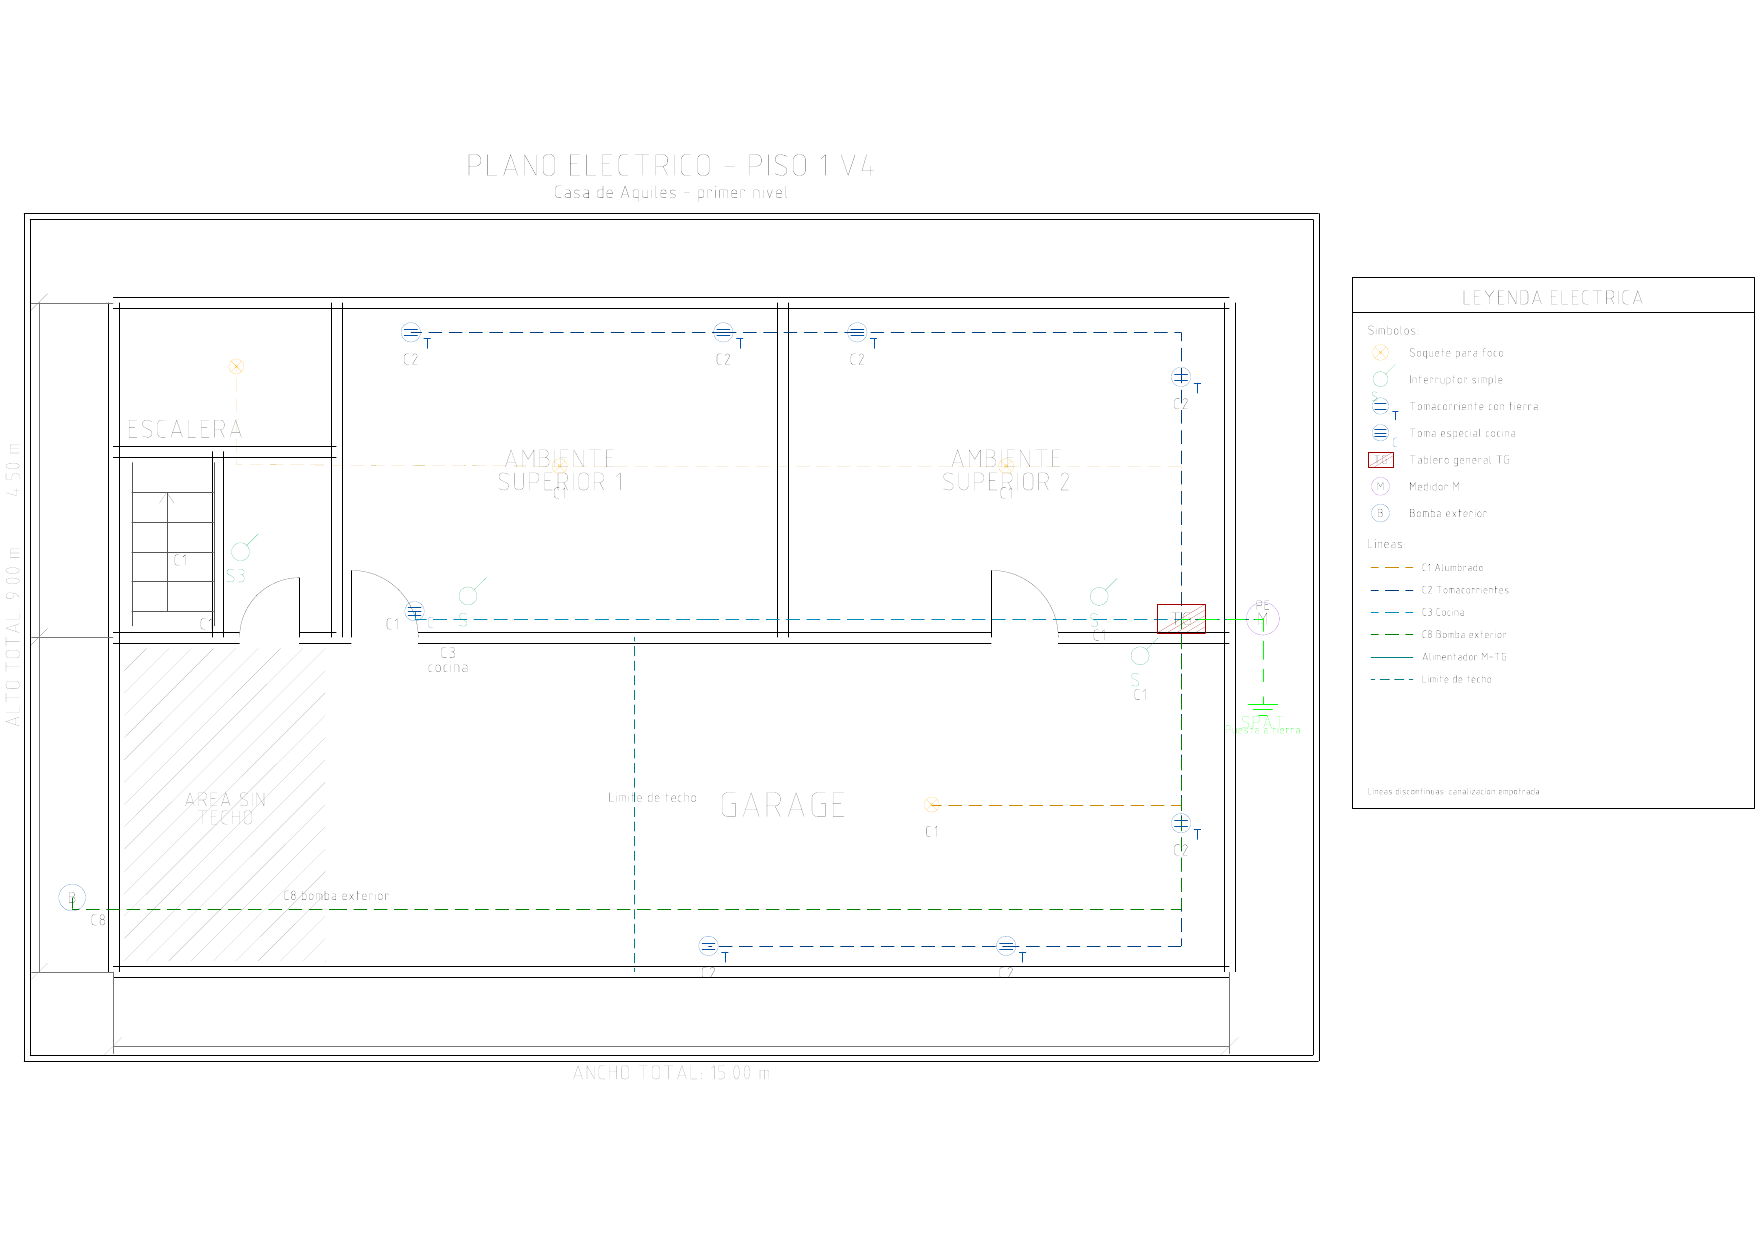
\includegraphics[height=0.70\textheight,keepaspectratio]{planos/plano_electrico_piso_1.png}
  \caption{Plano de Instalaciones Eléctricas - Primer Piso (vivienda de Aquiles)}
  \label{fig:plano-piso1}
\end{figure}
\end{landscape}

\subsection{IE-02: Plano de Instalaciones Eléctricas -- Segundo Piso}
Muestra la distribucion de los ambientes del segundo nivel, incluyendo el Tablero de Distribucion T2 alimentado desde el TG, los circuitos derivados de alumbrado, tomacorrientes generales, y las salidas especiales de cocina y lavadora.

\begin{landscape}
\begin{figure}[H]
  \centering
  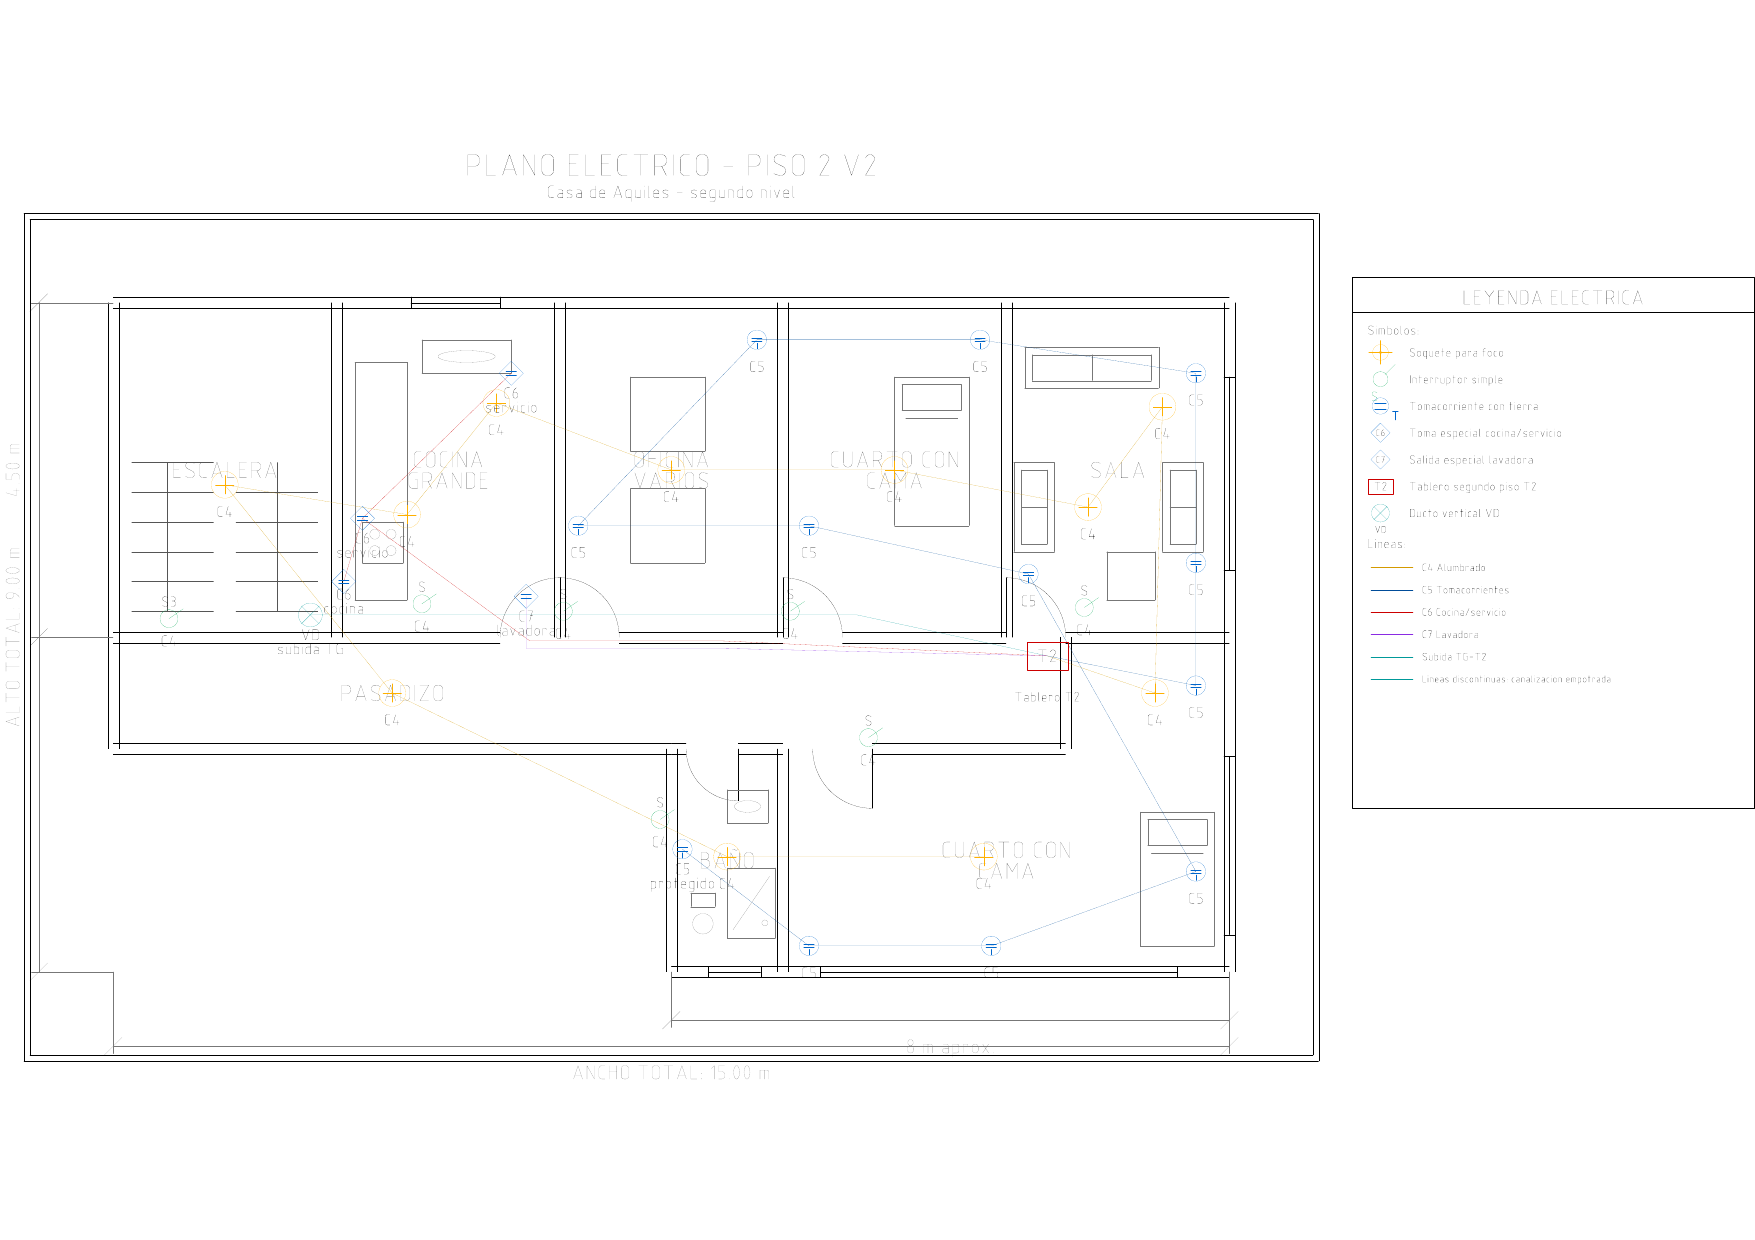
\includegraphics[height=0.70\textheight,keepaspectratio]{planos/plano_electrico_piso_2.png}
  \caption{Plano de Instalaciones Eléctricas - Segundo Piso (vivienda de Aquiles)}
  \label{fig:plano-piso2}
\end{figure}
\end{landscape}
